%***************************************************************************
% Chapter 4 of pluginarch.tex
% Authors: Remy Muller & Vincent Goudard
%***************************************************************************

\chapter{Control}

\noindent The control interface allow the user to act on parameters, to tune the behaviour of the audio processing function. This can be done in real-time, so that the user can directly hear the consequence of his changes on the audio signal transform.\\
\noindent There are different kinds of parameter, that require different handling. We can consider three main categories of parameters:
\begin{itemize}
\item{\textbf{Continuous parameters:}} These parameters can be characterized by the fact that they do not introduce a discontinuity in the audio stream \footnote{A dicontinuity in the audio stream is characterized by audible `zipper noise' or `clicks'}, when they change of a small amount. As a consequence, these parameters can be interpolated. These parameters are obviously represented by numerical values and can be considered `passive', in the sense that they are just used as a variable value in a generic computation. As examples: a filter's cutoff-frequency, a volume gain, a modulation frequency or a clipping threshold are continuous.

\item{\textbf{Events:}} These parameters, sometime referred to as \textbf{messages} or \textbf{commands}(EyesWeb), are characterized by their discrete nature. These messages can be of any type, but should belong to a set of predefined messages, known from the plugin. They are not directly used in computation, but are rather interpreted to trigger a specific action, without breaking the audio stream process. As examples: the choice between `sawtooth', `sine', and `square' for a modulator signal, a MIDI note-on event or the number of echoes in a delay.

\item{\textbf{Setup parameters:}} These parameters affects the plugin's configuration. They are non-realtime because they involve computationally expensive operations, like memory allocation, that definitely break the audio signal stream. As exemples: the choice of a impulse response file for a convolution plugin or a fft-size in a frequency domain transform.
\end{itemize}

\noindent This distinction between these three categories is not always that clear and well defined, but these three kinds of parameter correspond to different handlings.\\

\noindent With the increase of complexity of the plugins, which require more and more internal parameters to get finer acoustic results\footnote{e.g. in physical-modelling of instruments, reverb rooms...}, there is an ongoing need of mapping and conversion routines, so that the user can still control them in an ergonomic manner. The parameters available to the user and the host (\textbf{external parameters}) can differ from the parameters used in the process computation (\textbf{internal parameters}). There may exist a conversion layer between them.This conversion can be of various kind, such as scaling a gain expressed in dB to a linear scale, mapping of frequency, gain and resonance to filter coefficients or clipping of the parameter to its range.\\


%---------------------------------------------------------------------------
\section{External parameter declaration}
%...........................................................................
\subsection{Mandatory declarations}
\noindent The external parameters should be declared, to allow the host and/or the user to modify them. However, the host and the user do not need the same information to handle them.
The minimum required set of parameters properties that the host should know contains, at least, the two following:
\begin{itemize}
\item{\textbf{The parameter ID}}: This ID is used as a selector among the parameter structure. Parameters ID are signed or unsigned long integers in all major audio plugin standards, sometimes of an enumerated type (DXi, VST, RTAS).

\item{\textbf{The type}}: LADSPA and VST make use of 32-bit float only for all control data, and VST restrict the range to [0,1]. Other standards like DXi and AudioUnits implement all parameters as 32-bit float for efficiency, but keep a field in a parameter info structure, that defines whether to interpret the value as an integer, floating-point value, boolean, or enumeration (integer series). We find a similar mechanism in EyesWeb, but with three base format: double, int, and character string, plus a `Parameter type' flag.\\
% MAS : long, short, char, byte, bool, floatIEEE and float as text.
% RTAS ??
% !!!!! check that is is not fake like DX, and AU!!!!!
\end{itemize}


%...........................................................................
\subsection{Optional declarations}
\noindent Most plugin standards do offer much more information about parameters, to prevent the host and the user from manipulating them wrongly, and to let the user access them in a friendlier way. Such information may be stored in a `ParameterInfo' structure (DXi, AU), or suggested as defined flags or `hints' (LADSPA).

\begin{itemize}
\item{\textbf{The name or label}} is interesting for the user who do not speak like machines\ldots The parameter name can be part of a parameter information structure, like in DXi, EyesWeb and AU. LADSPA stores the port names (audio AND control) in an array. Parameter's name is not mandatory in VST, but a `GetParameterName' method exists in the API, that the developper can implement.
% MAS: ???

\item{\textbf{The units}} gives more sense to the values. Few standards offer this feature: DXi,and EyesWeb stores the unit of each parameter in the ParamInfo structure. In AU, the units is part of the type: for example the type `angle' is expressed in degrees or radians, the type `frequency' in Hertz\ldots and the parameter's mapping is chosen with respect to this.
% MAS : ????

\item{\textbf{The range}}: It gives hints about what values this parameter is assumed to take. This is useful to prevent the plugin from doing error-leading computations, like log(0), negative frequency for a filter \ldots etc. It also helps the user to grasp the meaning of the parameter he's handling. Almost all standards allow to specify the range of the parameters, except VST for which the range is normalized between [0;1] and conversion has to be done by hand. 

\item{\textbf{A default value}}: It can initialize the parameter to a relevant value, within the parameter range, at instantiation time. This feature is implemented in LADSPA, DXi, EyesWeb AU, MAS. In VST, it is stored in the default preset.
% RTAS :  ???

\item{\textbf{The mapping}}: It helps manipulating the parameter in a more ergonomic way. For example, frequency and gain are often more convenient when handled with logarithmic mapping. Mapping may be linear (all standards), logarithmic (LADSPA, AU), boolean (LADSPA, DXi, AU), indexed (LADSPA, DXi, AU)\ldots VST provides conversion tools for GUI-display only.
% EYESWEB : no mapping in the API

\item{\textbf{Automation\footnote{See \ref{automation} for explanation.}}}: Automatable parameters have to be declared as such by the apropriate mean:
\begin{itemize}
\item{AudioUnits}: Flag in the parameter information structure.
\item{DXi}: Index of automated parameters should be less than\\
\verb|NUM_AUTOMATED_PARAMS| within the parameters enumeration.
\item{MAS}: Automated parameters should be public.
\item{VST}: During run-time, one should use the specific method\\
\verb|setParameterAutomated|.
\end{itemize}
% RTAS : ??
\end{itemize}


\begin{table}
{\scriptsize
\begin{tabular}{|l|c|c|c|c|c|}
\hline
          & Name/Label        &  Units         & Range               & Default        & Mapping          \\
\hline
VST       &Not mandatory, but &  ---           & [0,1] fixed         & ---            & conversion tools \\
          & method in the API &                &                     &                & for display only \\
\hline
AU        & In a ParamInfo    & In a ParamInfo & Min, max stored in  & In a ParamInfo & Many many!       \\
          & structure         & structure      & ParamInfo struct    & structure      &                  \\
\hline
LADSPA    & In the PortNames  &  ---           & min and  max        & suggested as   & lin,log,int,     \\
          & array             &                & suggested as hints  & hint, relative & bool,SR-multiple \\
\hline
MAS       & ???               & ???            &  ???                & ???            & No               \\
\hline
DXi       & In a ParamInfo    & In a ParamInfo & Min, max stored in  & In a ParamInfo & ---              \\
          & structure         & structure      & ParamInfo struct    & structure      &                  \\
\hline
EyesWeb   & In a ParamInfo    & In a ParamInfo & Flags HAS\_MIN\/MAX & Yes            & ---              \\
          & structure         & structure      & and values          &                &                  \\
\hline
RTAS      & ???               & ???            &  ???                & ???            & ???              \\
\hline
\end{tabular}
}
\caption{Available parameter information}
\end{table}

\noindent Many other meta-information can be found in some standards:\\
\textbf{EyesWeb} specifies with the help of flags, whether the parameter can be changed at design-time, at runtime (and if so, if it can be exported), and if it is initially disabled.\\
\textbf{AudioUnits} provides a really rich API, with many predefined types of parameters, which have their own units, mapping, and range. This include indexed, boolean, percent, second, phase, cent, decibel, hertz, pan, a general type which is float between 0.0 and 1.0, and others. The developper can also add his own types.


%---------------------------------------------------------------------------
\section{Parameter update}
\noindent The parameter update mechanism should efficiently take in account the fact that the parameter update rate\footnote{There is no `rate' in the strict sense, but we used this word for convenience.} is asynchronous in nature, in general significantly lower than the audio stream, and that many changes could occur at the same time. Some parameters are known in advance (e.g. like MIDI events in a sequencer track), and some are not (e.g. live actualisation through hardware knobs). \\
The parameter update can be represented as a two steps operation: external parameters which have changed must be sent to the plugin; then, a conversion -- if necessary -- must make the corresponding internal parameters available to the process in a correct format. The figure \ref{parameters} illustrates this mechanism.

\begin{figure}[htb]
\begin{center}
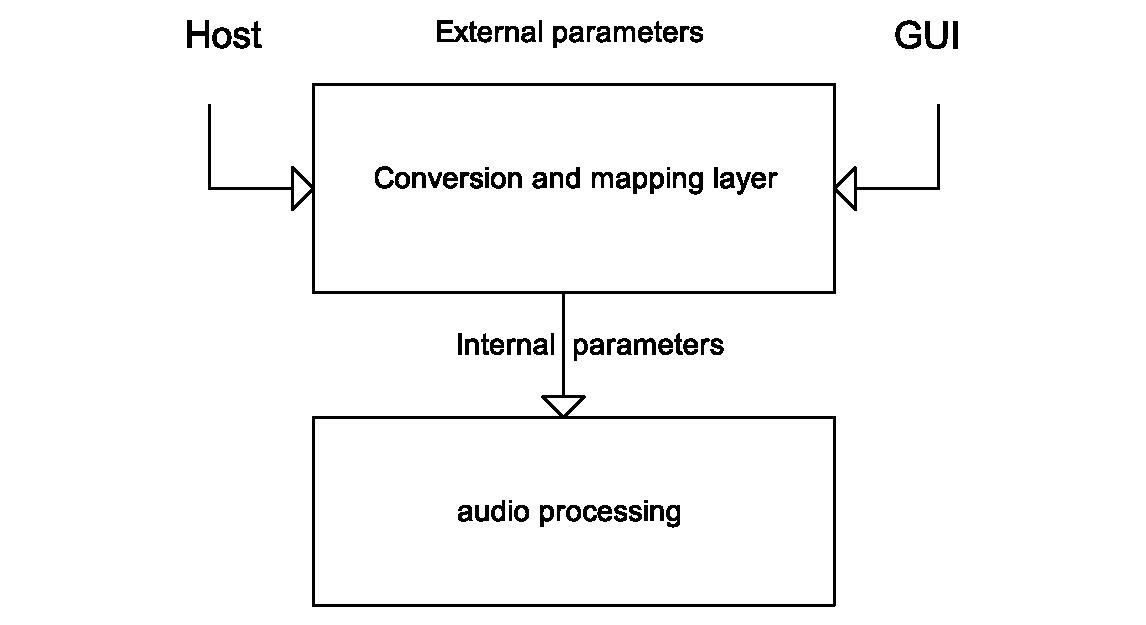
\includegraphics[height=3in,width=5in]{parameters}
\caption{Internal and external parameters}\label{parameters}
\end{center}
\end{figure}  

%...........................................................................
\subsection{Update mechanism}
% rate, sync/async, queues, timestamps ...

\noindent The most simple way to update parameters is the one implemented in LADSPA, and consists in a \textbf{polling mechanism}. At connection time, the host gives the plugin the adresses where it will write the external parameter values. The plugin can retrieve these values during the process function -- and only then --, assuming they may have changed. Everything that should be performed for mapping and conversion of these external parameters can only be done then.\\

\noindent In the second approach (VST, jMax), the host or the GUI calls a specific plugin method, usually called \verb|setParameter|. This method can only be called between two buffer processings. Necessary conversions and mappings should be implemented there by the plugin developer, so that internal parameters are up-to-date when the process function is called for the next buffer processing.\\

\noindent As a third case, some standards (DXi, AU) provide a conversion layer in the API between the plugin and the host or the GUI. Conversion and mapping are automatically done with the help of the parameter information structure. However, it is still necessary to retrieve the value of the parameters in the process function, and additionnal conversion have to be done here (e.g. computing filter coefficients from the cutoff frequency and the resonance, or checking mutual consistency of parameters).\\

\noindent Ways of handling events differ among plugin standards. A common and simple solution is to treat this set of value just like other parameters: reading and writing the value of the message with the \verb|GetParameter| and \verb|SetParameter| methods, and deciding on what should be done with a `\verb|case|' or `\verb|if|' condition. It can also be directly treated in the \verb|SetParameter| method (EyesWeb).



%...........................................................................
\subsection{Automation}
\label{automation}
\noindent The automation allow the user to record changes of parameters along a sequenced timeline, and play them back. These changes can be either recorded inline (i.e. in realtime, during playback) or offline (e.g. by editing graphically a curve on a sequenced track). The automation recording consists in taking the parameter's value every timeslice.\\
\noindent Most standards tends to allow this (DXi, AU, MAS, RTAS, VST) since it is a quite powerful tool. The parameters declared as automated parameters should be `realtime-able', i.e. they should not introduce too heavy computations or memory allocation. 

%...........................................................................
\subsection{Parameters encapsulation and meta data}

\noindent Some header-information might be provided to the plugin during runtime, in addition to the new parameter's value. Precisely, the time at which change occur, and the way the value should be modified can be specified.

\subsubsection{Type of data}
\noindent As it has been mentionned in the `Parameter declaration' section, some standard make use of a unique -or a restrained set of- data type for transport. In this case, a flag attached to the parameter in a parameter-info structure, specifies the type, into which the value should be casted.

\subsubsection{Timestamps}
\noindent The user who controls the interface can act at any time, disregarding what the plugin is doing. Thus, more than one change can occur during the time interval a timeslice is being processed. When considering punctual events such as audio attacks, synchronicity can play a major role in the audio rendition, and need more precision than the timeslice, which can last more than 50 ms.\\
\noindent Hence, timestamps can be attached to the parameter changes, to specify the precise sample accurate time at which they should occur. These events can be queued, their timestamp converted to the sample position within a buffer timeslice, and then be performed with the right time distribution during the next buffer processing.\\
\noindent In general, timestamping of parameters is limited to midi messages. Only EyesWeb make use of it for other control parameters.

\subsubsection{Interpolation}
\noindent On the other hand, for most parameters considered previously as `continuous', such a precision does not matter, since the audio timeslices are really small, but the continuous nature of the parameters should be respected to avoid `zipper noise' in the audio output signal. Therefore, various standards have implemented a way of interpolating the parameter' values to smooth the change, and avoid gaps in the audio stream that would generates these `clicks'. A common way of doing is to take in account the last value of the given parameter, and perform an interpolation between the new value and the previous one. Different kind of interpolation may be available to perform the interpolation such as linear (DXi, EyesWeb, AU) , quadratic (DXi) or sine (Dxi).\\
% TODO: which standard provide which interpolation?

% ---> What is given to the process function??   (derivative?, parameter buffer?)
% The DXi API  make use of the first and second derivative to interpolate the parameter's value between the bounds of the audio-buffer. Hence, the parameter's enveloppe is timestamped(?)\\
% EyesWeb modules provide a "Parameter smoothing" option.



%---------------------------------------------------------------------------
\section{Parameter persistence and presets}
\noindent Persistence of parameters is a saving of the parameters values, that enable the user to find these same values -- and not the default ones -- when the user re-open the plugin. It means that when the user close the host and relaunch it for a new session, the persistent parameters adjustments will be the same as when he quitted. This feature is useful when manipulating plugins with lots of control values, like an equalizer for example.\\
Presets are actually an extension of the persistence system to the user's will: the user can decide to store different sets of parameters that he likes, usually identifying them by a name. The way to store the preset depends on the presets size: if the preset is small, it can be stored by the host (VST) or in a register (DXi); whereas if the preset is bigger (e.g. it contains a waveform, or a picture), it will be stored in a separate file as a bytestream \footnote{The path of this file will be saved the same way a small preset would have been saved.}.\\


%---------------------------------------------------------------------------
\section{MIDI}
\noindent MIDI (Musical Instrument Digital Interface) is a protocol that transmits information about how music is produced. It is asynchronous but quantized at a maximum rate of 31,25 kbit/s\footnote{This rate was the standard for communication with hardware devices. However, hosts generally overcome this limitation internally: an adaptative resolution of 480 `ticks' per quarter-note is usual.}, and encode control values that fit in both \textit{event} (e.g. `note on/off') and \textit{continuous parameters} (e.g. `pitch bend') categories. As a major difference with GUI interaction, MIDI messages usually use time-stamps, allowing sample accurate rendering. One can distinguish different families among musical plugins using MIDI: synthesizers, MIDI-controlled effects, pure MIDI effects\footnote{MIDI effects consist in taking MIDI messages as data input and process them. No audio data is implied in the process. Most common MIDI effects are arpegiators, delays and echoes\ldots} and analysis plugins -- though those last ones aren't formalized in any standard for now -- depending on the kind of input and output data. In this document, we will only deal with synthesizers and MIDI-controlled effects.\\

%...........................................................................
\subsection{Synthesizers}
\noindent Synthesizers (or `instruments') appeared in the second generation of plugin standards. As harware ones, they get MIDI messages as input, usually have no audio input, and output audio data on many pins compared to chained effects. They often have a lot more parameters, and many of these ones are mapped to MIDI continuous controllers for a convenient live interaction.

%...........................................................................
\subsection{MIDI-controlled effects}
\noindent Integration of synthetizers into standards has allowed the interaction with plugins via MIDI. It allows to `play' an effect as an intrument, using the incoming audio as a primary material to generate sound. They are often intented for musicians more than sound-engineers. As examples we can cite filters whose cut-off frequency is tuned to MIDI notes, or live-samplers using the incoming audio as a wave-table.
%----------------------------------EOF-------------------------------------%
